\documentclass[journal,12pt,twocolumn]{IEEEtran}

\usepackage{setspace}
\usepackage{gensymb}
\singlespacing
\usepackage[cmex10]{amsmath}

\usepackage{amsthm}

\usepackage{mathrsfs}
\usepackage{txfonts}
\usepackage{stfloats}
\usepackage{bm}
\usepackage{cite}
\usepackage{cases}
\usepackage{subfig}

\usepackage{longtable}
\usepackage{multirow}

\usepackage{enumitem}
\usepackage{mathtools}
\usepackage{steinmetz}
\usepackage{tikz}
\usepackage{circuitikz}
\usepackage{verbatim}
\usepackage{tfrupee}
\usepackage[breaklinks=true]{hyperref}
\usepackage{graphicx}
\usepackage{tkz-euclide}

\usetikzlibrary{calc,math}
\usepackage{listings}
    \usepackage{color}                                            %%
    \usepackage{array}                                            %%
    \usepackage{longtable}                                        %%
    \usepackage{calc}                                             %%
    \usepackage{multirow}                                         %%
    \usepackage{hhline}                                           %%
    \usepackage{ifthen}                                           %%
    \usepackage{lscape}     
\usepackage{multicol}
\usepackage{chngcntr}

\DeclareMathOperator*{\Res}{Res}

\renewcommand\thesection{\arabic{section}}
\renewcommand\thesubsection{\thesection.\arabic{subsection}}
\renewcommand\thesubsubsection{\thesubsection.\arabic{subsubsection}}

\renewcommand\thesectiondis{\arabic{section}}
\renewcommand\thesubsectiondis{\thesectiondis.\arabic{subsection}}
\renewcommand\thesubsubsectiondis{\thesubsectiondis.\arabic{subsubsection}}


\hyphenation{op-tical net-works semi-conduc-tor}
\def\inputGnumericTable{}                                 %%

\lstset{
%language=C,
frame=single, 
breaklines=true,
columns=fullflexible
}
\begin{document}


\newtheorem{theorem}{Theorem}[section]
\newtheorem{problem}{Problem}
\newtheorem{proposition}{Proposition}[section]
\newtheorem{lemma}{Lemma}[section]
\newtheorem{corollary}[theorem]{Corollary}
\newtheorem{example}{Example}[section]
\newtheorem{definition}[problem]{Definition}

\newcommand{\BEQA}{\begin{eqnarray}}
\newcommand{\EEQA}{\end{eqnarray}}
\newcommand{\define}{\stackrel{\triangle}{=}}
\bibliographystyle{IEEEtran}
\raggedbottom
\setlength{\parindent}{0pt}
\providecommand{\mbf}{\mathbf}
\providecommand{\pr}[1]{\ensuremath{\Pr\left(#1\right)}}
\providecommand{\qfunc}[1]{\ensuremath{Q\left(#1\right)}}
\providecommand{\sbrak}[1]{\ensuremath{{}\left[#1\right]}}
\providecommand{\lsbrak}[1]{\ensuremath{{}\left[#1\right.}}
\providecommand{\rsbrak}[1]{\ensuremath{{}\left.#1\right]}}
\providecommand{\brak}[1]{\ensuremath{\left(#1\right)}}
\providecommand{\lbrak}[1]{\ensuremath{\left(#1\right.}}
\providecommand{\rbrak}[1]{\ensuremath{\left.#1\right)}}
\providecommand{\cbrak}[1]{\ensuremath{\left\{#1\right\}}}
\providecommand{\lcbrak}[1]{\ensuremath{\left\{#1\right.}}
\providecommand{\rcbrak}[1]{\ensuremath{\left.#1\right\}}}
\theoremstyle{remark}
\newtheorem{rem}{Remark}
\newcommand{\sgn}{\mathop{\mathrm{sgn}}}
\providecommand{\abs}[1]{\left\vert#1\right\vert}
\providecommand{\res}[1]{\Res\displaylimits_{#1}} 
\providecommand{\norm}[1]{\left\lVert#1\right\rVert}
%\providecommand{\norm}[1]{\lVert#1\rVert}
\providecommand{\mtx}[1]{\mathbf{#1}}
\providecommand{\mean}[1]{E\left[ #1 \right]}
\providecommand{\fourier}{\overset{\mathcal{F}}{ \rightleftharpoons}}
%\providecommand{\hilbert}{\overset{\mathcal{H}}{ \rightleftharpoons}}
\providecommand{\system}{\overset{\mathcal{H}}{ \longleftrightarrow}}
	%\newcommand{\solution}[2]{\textbf{Solution:}{#1}}
\newcommand{\solution}{\noindent \textbf{Solution: }}
\newcommand{\cosec}{\,\text{cosec}\,}
\providecommand{\dec}[2]{\ensuremath{\overset{#1}{\underset{#2}{\gtrless}}}}
\newcommand{\myvec}[1]{\ensuremath{\begin{pmatrix}#1\end{pmatrix}}}
\newcommand{\mydet}[1]{\ensuremath{\begin{vmatrix}#1\end{vmatrix}}}
\numberwithin{equation}{subsection}

\makeatletter
\@addtoreset{figure}{problem}
\makeatother
\let\StandardTheFigure\thefigure
\let\vec\mathbf

\renewcommand{\thefigure}{\theproblem}

\def\putbox#1#2#3{\makebox[0in][l]{\makebox[#1][l]{}\raisebox{\baselineskip}[0in][0in]{\raisebox{#2}[0in][0in]{#3}}}}
     \def\rightbox#1{\makebox[0in][r]{#1}}
     \def\centbox#1{\makebox[0in]{#1}}
     \def\topbox#1{\raisebox{-\baselineskip}[0in][0in]{#1}}
     \def\midbox#1{\raisebox{-0.5\baselineskip}[0in][0in]{#1}}
\vspace{3cm}
\title{Problem Linman 3.6.3}
\author{Sachinkumar Dubey - EE20MTECH11009}
\maketitle
\newpage
\bigskip

\section{Problem}
What conic does the following equation represent.
\begin{align}
9y^2-24xy+16x^2-18x-101y+19=0
\end{align}
Find the center and equation refered to centre.
\section{Solution}
The general second degree equation can be expressed as follows,
\begin{align}
\Vec{x}^T\Vec{V}\Vec{x}+2\Vec{u}^T\Vec{x}+f=0
\intertext{where,}
\vec{V} &= \myvec{9&-12\\-12&16}\\ \label{eq:conics/ex/solution/given1}
\vec{u} &= \myvec{-9\\-\frac{101}{2}}\\ 
f &= 19 \label{eq:conics/ex/solution/given2}
\end{align}
\begin{enumerate}
\item Expanding the determinant of $\vec{V}$ we observe, 
\begin{align}
\mydet{9&-12\\-12&16} = 0 \label{eq:conics/ex/solution/eq2.1}
\end{align}
Also
\begin{align}
    \mydet{\vec{V} & \vec{u} \\ \vec{u}^T & f}=
    \mydet{9&-12 & -9 \\-12&16 & -\frac{101}{2} \\ -9 & -\frac{101}{2} & 19} \\
    \neq 0\label{eq:conics/ex/solution/eq2.2}
\end{align}
Hence from \eqref{eq:conics/ex/solution/eq2.1} and \eqref{eq:conics/ex/solution/eq2.2} we conclude that given equation is an parabola. The characteristic equation of $\vec{V}$ is given as follows,
\begin{align}
\mydet{\lambda\vec{I}-\vec{V}} = \mydet{\lambda-9&12\\12&\lambda-16} &= 0\\
\implies \lambda^2-25\lambda &= 0\label{eq:conics/ex/solution/eqchar}
\end{align}
Hence the characteristic equation of $\vec{V}$ is given by \eqref{eq:conics/ex/solution/eqchar}. The roots of \eqref{eq:conics/ex/solution/eqchar} i.e the eigenvalues are given by
\begin{align}
\lambda_1=0, \lambda_2=25\label{eq:conics/ex/solution/eqeigenvals}    
\end{align}
\item For $\lambda_1 = 0$, the eigen vector $\vec{p}$ is given by 
\begin{align}
\vec{V}\vec{p} = 0
\end{align}
Row reducing $\vec{V}$ yields
\begin{align}
\implies
\myvec{-9&12\\12&-16}\xleftrightarrow[R_2=R_2+4R_1]{R_1=-\frac{R_1}{3}}\myvec{3&-4\\0&0}\\
\implies\vec{p}_1=\frac{1}{5}\myvec{-4\\-3} \label{eq:conics/ex/solution/eq2.3}
\end{align}
Similarly, 
\begin{align}
\vec{p}_2=\frac{1}{5}\myvec{-3\\4} 
\end{align}
%
Thus, the eigenvector rotation matrix and the eigenvalue matrix are
\begin{align}
\vec{P}&=\myvec{\vec{p_1}&\vec{p_2}}=\frac{1}{5}\myvec{-4&-3\\ -3 &4} \\
\vec{D}&=\myvec{0&0\\0&25}
\end{align}
The focal length of the parabola is given by 
\begin{align}
\frac{\abs{2\vec{u}^T\vec{p_1}}}{\lambda_2}
    = \frac{75}{25}=3
\end{align}
and its equation is
\begin{align}
    \vec{y^T}\vec{D}\vec{y}&=-\eta\myvec{1&0}\vec{y}\label{eq:conics/ex/solution/eq2.4}
\end{align}
where
\begin{align}
    \eta=2\vec{u}^T\vec{p_1}=75
\end{align}
and the vertex $\vec{c}$ is given by 
\begin{align}
    \myvec{\vec{u^T}+\frac{\eta}{2}\vec{p_1^T} \\ \vec{V}}\vec{c}=
    \myvec{-f \\\frac{\eta}{2}\vec{p_1}-\vec{u}} 
\end{align}
using equations \eqref{eq:conics/ex/solution/given1},\eqref{eq:conics/ex/solution/given2} and \eqref{eq:conics/ex/solution/eq2.3}
\begin{align}
    \myvec{-39& -73 \\ 9 & -12 \\  -12 & 16 }\vec{c}=\myvec{-19 \\ -21\\ 28} \label{eq:conics/ex/solution/eqcen}
\end{align}
Forming the augmented matrix and row reducing it:
\begin{align}
\myvec{-39 & -73 & -19\\9 & -12 & -21 \\-12 & 16 &28 }\\
R_3\leftrightarrow R_3+(4/3)R_2 \nonumber \\
\myvec{-39 & -73 & -19\\9 & -12 & -21 \\0 & 0 &0 }\\
R_1\leftrightarrow R_1/(-39) \nonumber \\
\myvec{1 & 73/39 & 19/39\\9 & -12 & -21 \\0 & 0 &0 }\\
R_2\leftrightarrow R_2-9R_1 \nonumber \\
\myvec{1 & 73/39 & 19/39\\0 & -1125/39 & -990/39 \\0 & 0 &0}\\ R_2\leftrightarrow R_2 \times (-39/1125) \nonumber \\
\myvec{1 & 73/39 & 19/39\\0 & 1 & 22/25 \\0 & 0 &0}\\
R_1\leftrightarrow R_1 -(73/39)R_2 \nonumber \\
\myvec{1 & 0 & -29/25\\0 & 1 & 22/25 \\0 & 0 &0}
\end{align}
Thus the vertex $\vec{c}$ is:
\begin{align}
\vec{c}=\myvec{ -29/25\\22/25}= \myvec{-1.16\\ 0.88} 
\end{align}
\begin{figure}[h!]
    \centering
    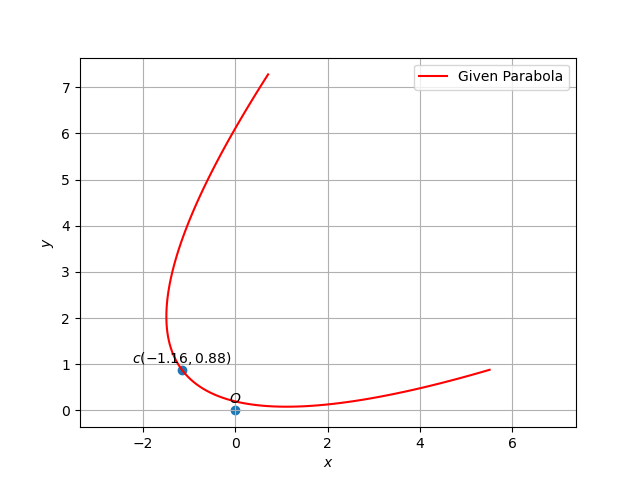
\includegraphics[width=10cm]{Figure_1.png}
    \caption{Plot of the Parabola and its vertex}
    \label{Plot of the Asymtotes}
\end{figure}
\end{document}